% =====================================================================
%  Rapport de projet de Machine Learning
%  Développement d'un assistant multi-agent pour la sélection
%  intelligente des portefeuilles financiers
%
%  Compilation : pdflatex rapport.tex (deux fois, pour la table des matières)
%  Overleaf    : importer le dossier docs/rapport/ (rapport.tex, chiffres.tex, tab_*.tex, figures/)
%  Les chiffres et figures viennent de generer_figures.py : relancer ce script
%  après un vrai cycle (Ollama + yfinance) puis recompiler.
% =====================================================================
\documentclass[11pt,a4paper]{report}

% ---------------------------------------------------------------- à compléter
\newcommand{\Ecole}{[Nom de l'école]}
\newcommand{\Filiere}{[Filière / Master]}
\newcommand{\Auteurs}{[Prénom NOM]\\[2pt][Prénom NOM]\\[2pt][Prénom NOM]}
\newcommand{\Encadrant}{[Prénom NOM]}
\newcommand{\Annee}{Année universitaire 2026--2027}

% ---------------------------------------------------------------- paquets
\usepackage[T1]{fontenc}
\usepackage[utf8]{inputenc}
\usepackage[french]{babel}
\usepackage{mathpazo}
\usepackage[scaled=0.92]{helvet}
\usepackage{microtype}
\usepackage[a4paper,margin=2.5cm,headheight=14pt]{geometry}
\usepackage{amsmath,amssymb}
\usepackage{graphicx}
\usepackage{booktabs,tabularx,longtable,array}
\usepackage{xcolor}
\usepackage{tikz}
\usetikzlibrary{positioning,arrows.meta,shapes.geometric,fit,calc,backgrounds}
\usepackage[most]{tcolorbox}
\usepackage{listings}
\usepackage{enumitem}
\usepackage{titlesec}
\usepackage{fancyhdr}
\usepackage{caption}
\usepackage{float}
\usepackage[hidelinks]{hyperref}

% ---------------------------------------------------------------- identité visuelle
\definecolor{encre}{HTML}{0E3B43}
\definecolor{laiton}{HTML}{B0802A}
\definecolor{ardoise}{HTML}{5B6670}
\definecolor{filet}{HTML}{DADDD8}
\definecolor{fond}{HTML}{F1F3EF}
\definecolor{code}{HTML}{2A78D6}
\definecolor{llm}{HTML}{6250D6}
\definecolor{humain}{HTML}{E07B2E}
\hypersetup{colorlinks=true,linkcolor=encre,citecolor=laiton,urlcolor=encre}

\titleformat{\chapter}[display]{\sffamily\color{encre}}
  {\large\color{laiton}\bfseries Chapitre~\thechapter}{4pt}{\Huge\bfseries}
  [\vspace{2pt}{\color{filet}\titlerule[0.8pt]}]
\titlespacing*{\chapter}{0pt}{-10pt}{24pt}
\titleformat{\section}{\sffamily\Large\bfseries\color{encre}}{\color{laiton}\thesection}{0.8em}{}
\titleformat{\subsection}{\sffamily\large\bfseries\color{encre}}{\color{laiton}\thesubsection}{0.8em}{}
\captionsetup{font=small,labelfont={bf,color=encre},labelsep=period}

\pagestyle{fancy}
\fancyhf{}
\fancyhead[L]{\small\sffamily\color{ardoise}Assistant multi-agent de sélection de portefeuille}
\fancyhead[R]{\small\sffamily\color{ardoise}\leftmark}
\fancyfoot[C]{\small\sffamily\thepage}
\renewcommand{\headrulewidth}{0.4pt}
\renewcommand{\headrule}{{\color{filet}\hrule width\headwidth height\headrulewidth}}
\renewcommand{\chaptermark}[1]{\markboth{#1}{}}

\newtcolorbox{retenir}[1][À retenir]{colback=fond,colframe=encre,boxrule=0pt,leftrule=3pt,
  arc=0pt,left=10pt,right=10pt,top=6pt,bottom=6pt,fonttitle=\sffamily\bfseries,coltitle=encre,
  title={#1},attach title to upper={\par\smallskip},before upper={}}

\lstset{basicstyle=\ttfamily\small,backgroundcolor=\color{fond},frame=leftline,rulecolor=\color{encre},
  framerule=2pt,xleftmargin=8pt,breaklines=true,columns=fullflexible,keepspaces=true,
  commentstyle=\color{ardoise},keywordstyle=\color{encre}\bfseries,showstringspaces=false,
  literate={é}{{\'e}}1 {è}{{\`e}}1 {à}{{\`a}}1 {ê}{{\^e}}1 {ç}{{\c{c}}}1 {ô}{{\^o}}1 {É}{{\'E}}1
           {├}{{+}}1 {└}{{+}}1 {─}{{-}}1 {│}{{|}}1}

\setlist{itemsep=2pt,topsep=4pt}
\setlength{\emergencystretch}{3em}
\DeclareUnicodeCharacter{2212}{\ensuremath{-}}
\newcolumntype{Y}{>{\raggedright\arraybackslash}X}

% \input n'est pas utilisable au milieu d'un tableau : on passe par la primitive
\makeatletter\newcommand{\tabinput}[1]{\@@input #1 }\makeatother

% chiffres du dernier cycle exporté (generer_figures.py)
% généré par generer_figures.py
\newcommand{\DateAnalyse}{20 novembre 2026}
\newcommand{\RendementAttendu}{13{,}5\,\%}
\newcommand{\Volatilite}{17{,}2\,\%}
\newcommand{\Sharpe}{0{,}55}
\newcommand{\NbLignes}{25}
\newcommand{\VaR}{1{,}75\,\%}
\newcommand{\CVaR}{2{,}20\,\%}
\newcommand{\Rotation}{73\,\%}
\newcommand{\NbEligibles}{50}
\newcommand{\NbNotes}{150}
\newcommand{\NbSelection}{25}
\newcommand{\NbIterations}{2}
\newcommand{\Conforme}{conforme}
\newcommand{\Moteur}{scipy (repli)}
\newcommand{\BackendLLM}{mock}
\newcommand{\SourceDonnees}{synthetic}
\newcommand{\PerfPortefeuille}{$-$9{,}3\,\%}
\newcommand{\PerfIndice}{$-$0{,}4\,\%}
\newcommand{\PireStress}{20{,}8\,\%}
\newcommand{\VersionDonnees}{9daba6e981bc}


% =====================================================================
\begin{document}

% ---------------------------------------------------------------- page de garde
\begin{titlepage}
\newgeometry{margin=2.2cm}
\sffamily
{\color{ardoise}\large \Ecole\par \Filiere\par}
\vspace{3.2cm}
{\color{laiton}\large\bfseries Projet de Machine Learning\par}
\vspace{10pt}
{\color{encre}\fontsize{27}{33}\selectfont\bfseries Développement d'un assistant multi-agent pour la sélection intelligente des portefeuilles financiers\par}
\vspace{14pt}
{\color{ardoise}\Large Le LLM analyse, le code calcule, le gérant décide.\par}
\vspace{1.6cm}
\begin{tikzpicture}
  % bande d'allocation stylisée (motif de l'interface)
  \foreach \x/\w/\c in {0/3.2/E87BA4,3.25/2.8/1BAF7A,6.1/2.5/EDA100,8.65/2.4/2A78D6,11.1/1.1/EB6834,12.25/0.6/008300,12.9/0.35/6250D6}
    {\definecolor{tmp}{HTML}{\c}\fill[tmp] (\x,0) rectangle ++(\w,0.55);}
\end{tikzpicture}
\vfill
\begin{minipage}[t]{0.48\textwidth}
{\color{ardoise}Réalisé par}\par\vspace{4pt}{\color{encre}\large\Auteurs\par}
\end{minipage}\hfill
\begin{minipage}[t]{0.48\textwidth}
{\color{ardoise}Encadré par}\par\vspace{4pt}{\color{encre}\large\Encadrant\par}
\end{minipage}
\vspace{1.2cm}
{\color{filet}\rule{\textwidth}{0.6pt}}\par
{\color{ardoise}\Annee}
\restoregeometry
\end{titlepage}

% ---------------------------------------------------------------- pages liminaires
\pagenumbering{roman}
\chapter*{Résumé}
\addcontentsline{toc}{chapter}{Résumé}
Ce projet développe un assistant d'aide à la décision qui sélectionne des actions et construit un portefeuille
pour un gérant, en combinant des agents fondés sur de grands modèles de langage (LLM) et des méthodes
quantitatives éprouvées. Inspiré du cadre \emph{TradingAgents}~\cite{tradingagents}, le système est orchestré
par LangGraph en neuf étapes : construction de l'univers selon le mandat, collecte de données point-in-time,
calcul de facteurs standardisés, analyse de chaque titre par trois agents LLM en parallèle (fondamental,
sentiment, valorisation), débat entre un chercheur haussier et un chercheur baissier arbitré par un juge,
optimisation Black-Litterman sous contraintes avec une covariance de Ledoit-Wolf, contrôle des risques
(VaR, CVaR, stress tests) avec au plus trois ajustements, validation humaine, puis rédaction d'une note
d'investissement et d'un journal d'audit.

Le principe directeur est une séparation stricte des rôles : les modèles de langage interprètent
l'information et formulent des vues qualitatives, mais aucun chiffre (métrique, rendement attendu,
pondération) n'est produit par un LLM. Le système est entièrement open source (Qwen2.5 via Ollama,
LangGraph, PyPortfolioOpt), observable avec LangSmith et utilisable via une interface Streamlit.

\medskip\noindent\textbf{Mots-clés :} systèmes multi-agents, grands modèles de langage, LangGraph,
optimisation de portefeuille, Black-Litterman, estimation de covariance par rétrécissement, gestion des risques.

\chapter*{Abstract}
\addcontentsline{toc}{chapter}{Abstract}
This project builds a decision-support assistant that selects equities and constructs a portfolio for a
portfolio manager by combining large language model (LLM) agents with established quantitative methods.
Inspired by the \emph{TradingAgents} framework, a nine-step LangGraph workflow builds a mandate-compliant
universe, collects point-in-time data, computes standardised factors, runs three parallel LLM analysts per stock,
holds a bull-versus-bear debate settled by a judge, optimises weights with Black-Litterman and Ledoit-Wolf
shrinkage under mandate constraints, checks risk with up to three adjustment rounds, pauses for human
approval, and writes an investment note with a full audit trail. LLMs interpret; code computes; the manager decides.

\medskip\noindent\textbf{Keywords:} multi-agent systems, large language models, LangGraph, portfolio optimisation,
Black-Litterman, shrinkage covariance estimation, risk management.

\tableofcontents
\listoffigures
\listoftables

\cleardoublepage
\pagenumbering{arabic}

% =====================================================================
\chapter{Introduction}

\section{Contexte}
La gestion de portefeuille consiste à répartir un capital entre des actifs de manière à obtenir le meilleur
rendement possible pour un niveau de risque accepté. Depuis Markowitz~\cite{markowitz}, cette décision
s'appuie sur des estimations de rendements et de covariances. En pratique, un gérant mobilise aussi une
information qualitative abondante : rapports annuels, actualités, opinions d'analystes. Les grands modèles
de langage savent désormais lire et résumer ce type d'information~\cite{finbert,bloomberggpt}, et les
architectures d'agents leur permettent d'utiliser des outils et de raisonner par étapes~\cite{react}.

\section{Problématique}
Comment exploiter la capacité d'analyse des LLM pour sélectionner des titres, sans leur confier ce qu'ils
font mal (calculer, rester cohérents dans le temps, respecter des contraintes chiffrées) et sans retirer au
gérant la responsabilité de la décision ? La question se décline en trois sous-questions :
\begin{enumerate}
  \item comment organiser plusieurs agents spécialisés pour qu'ils produisent un avis fiable et traçable ;
  \item comment transformer des avis qualitatifs en pondérations optimales et conformes au mandat ;
  \item comment garantir le contrôle du risque et la supervision humaine à chaque cycle.
\end{enumerate}

\section{Objectifs}
\begin{itemize}
  \item Concevoir une architecture multi-agent orchestrée par LangGraph, fidèle au processus d'un comité d'investissement.
  \item Combiner des agents LLM (analyse, débat, arbitrage) avec des modèles quantitatifs (facteurs, Ledoit-Wolf, Black-Litterman).
  \item Respecter un mandat de gestion (plafonds par titre et par secteur, liquidité, limites de risque).
  \item Rendre chaque décision traçable et observable, et la soumettre à la validation du gérant.
  \item Livrer un prototype gratuit et open source, exécutable sur Google Colab.
\end{itemize}

\section{Organisation du rapport}
Le chapitre~\ref{ch:etat} présente l'état de l'art. Le chapitre~\ref{ch:archi} décrit l'architecture et les
hypothèses de travail. Les chapitres~\ref{ch:donnees} à~\ref{ch:optim} détaillent les données, les agents et
l'optimisation. Le chapitre~\ref{ch:impl} décrit l'implémentation, le chapitre~\ref{ch:resultats} présente une
démonstration, et le chapitre~\ref{ch:limites} discute les limites et perspectives.

% =====================================================================
\chapter{État de l'art}\label{ch:etat}

\section{Théorie moderne du portefeuille}
Markowitz~\cite{markowitz} formalise le choix d'un portefeuille $w\in\mathbb{R}^n$ comme un arbitrage entre
rendement espéré $w^\top\mu$ et variance $w^\top\Sigma w$. La qualité d'un portefeuille est souvent résumée par
le ratio de Sharpe~\cite{sharpe} :
\begin{equation}
  S(w) = \frac{w^\top \mu - r_f}{\sqrt{w^\top \Sigma w}},
\end{equation}
où $r_f$ est le taux sans risque. La difficulté principale est l'estimation : de petites erreurs sur $\mu$ produisent
des portefeuilles extrêmes et instables.

\section{Estimation de la covariance par rétrécissement}
Avec $n$ actifs et $T$ observations, la covariance empirique $S$ est bruitée lorsque $n$ n'est pas négligeable
devant $T$. Ledoit et Wolf~\cite{ledoitwolf} proposent un estimateur rétréci, combinaison convexe d'une cible
structurée $F$ et de $S$ :
\begin{equation}
  \hat\Sigma = \delta^\star F + (1-\delta^\star) S,
\end{equation}
où l'intensité $\delta^\star$ minimise analytiquement l'erreur quadratique attendue. C'est un exemple classique
de compromis biais-variance, au cœur de l'apprentissage statistique.

\section{Le modèle de Black-Litterman}
Black et Litterman~\cite{blacklitterman} partent des rendements implicites du marché
$\pi = \delta\,\Sigma\,w_{\text{mkt}}$ (équilibre) et les combinent, de façon bayésienne, avec des vues
$Q = P\mu + \varepsilon$, $\varepsilon\sim\mathcal{N}(0,\Omega)$. Le rendement a posteriori est :
\begin{equation}
  \mu_{BL} = \left[(\tau\Sigma)^{-1} + P^\top\Omega^{-1}P\right]^{-1}\left[(\tau\Sigma)^{-1}\pi + P^\top\Omega^{-1}Q\right].
\end{equation}
Idzorek~\cite{idzorek} relie l'incertitude $\Omega$ à une confiance exprimée en pourcentage, ce qui rend
le modèle utilisable avec des vues qualitatives, exactement ce que produisent nos agents.

\section{Mesures de risque}
La valeur en risque (VaR) au niveau $\alpha$ est le quantile des pertes ; la CVaR (ou Expected Shortfall) est la perte
moyenne au-delà de la VaR et constitue une mesure cohérente~\cite{cvar}. Les stress tests complètent ces mesures
en évaluant la perte sous des scénarios extrêmes.

\section{Modèles de langage et finance}
FinBERT~\cite{finbert} a montré l'intérêt de modèles de langage spécialisés pour l'analyse de sentiment financier,
et BloombergGPT~\cite{bloomberggpt} celui de modèles génératifs entraînés sur des corpus financiers.
Les modèles ouverts récents, comme Qwen2.5~\cite{qwen}, atteignent un niveau suffisant pour l'extraction
d'information et la rédaction, et peuvent être exécutés localement. La génération augmentée par recherche
(RAG)~\cite{rag} permet d'ancrer leurs réponses dans des documents (rapports annuels).

\section{Agents LLM et systèmes multi-agents}
ReAct~\cite{react} combine raisonnement et appels d'outils. \emph{TradingAgents}~\cite{tradingagents}
reproduit la structure d'une société de trading : analystes spécialisés, chercheurs haussier et baissier en débat,
trader et gestion du risque. Notre projet reprend cette idée de rôles et de débat, mais l'applique à la construction
de portefeuille et la combine à une optimisation quantitative et à une validation humaine.
LangGraph~\cite{langgraph} fournit les briques d'orchestration : graphe d'états, exécution parallèle,
points de reprise et interruption pour intervention humaine.

% =====================================================================
\chapter{Cadrage et architecture}\label{ch:archi}

\section{Principe directeur}
\begin{retenir}[{Le LLM analyse, le code calcule, le gérant décide}]
Les agents LLM lisent, interprètent et argumentent ; ils produisent des notes et des vues qualitatives.
Toutes les grandeurs numériques (métriques, rendements attendus, pondérations, mesures de risque) sont calculées
par du code déterministe. Aucune décision n'est appliquée sans l'accord explicite du gérant.
\end{retenir}

\section{Hypothèses de travail}
Le tableau~\ref{tab:hyp} liste les hypothèses définies avec l'équipe, à valider avec les gérants.

\begin{table}[H]
\centering\small
\caption{Hypothèses de travail et leur traduction dans le système}\label{tab:hyp}
\begin{tabularx}{\textwidth}{@{}l l Y@{}}
\toprule
& Hypothèse & Traduction dans le système \\
\midrule
H1 & Aide à la décision & Interruption du graphe avant toute conclusion ; ordres à passer manuellement. \\
H2 & Actions long-only & Univers d'un indice de référence (50 à 300 titres), pas de vente à découvert. \\
H3 & Fréquence mensuelle & Un cycle par mois, identifié par un \texttt{thread\_id}. \\
H4 & Objectif & Maximiser le ratio de Sharpe ; comparaison à l'indice. \\
H5 & Mandat & 10\,\% max par titre, 30\,\% max par secteur, liquidité minimale. \\
H6 & Données & Prix quotidiens sur 3 ans ou plus, états financiers, actualités. \\
H7 & Règle d'or & Le LLM ne produit aucun chiffre. \\
H8 & Point-in-time & Aucune information postérieure à la date d'analyse. \\
H9 & Boucle de risque & Trois tentatives d'ajustement au maximum, puis escalade au gérant. \\
H10 & Traçabilité & Thèses, sources, versions des données et du mandat journalisées. \\
\bottomrule
\end{tabularx}
\end{table}

\section{Workflow en neuf étapes}
La figure~\ref{fig:workflow} présente le flux. Chaque étape est de type \emph{code} (déterministe),
\emph{LLM} (agents) ou \emph{humain}.

\begin{figure}[H]
\centering
\begin{tikzpicture}[
  every node/.style={font=\sffamily\footnotesize},
  etape/.style={rectangle,rounded corners=2pt,minimum width=2.55cm,minimum height=1.25cm,align=center,text=white},
  fl/.style={-{Stealth[length=2.2mm]},thick,color=ardoise}]
  \node[etape,fill=code]   (e1) {\textbf{1} Construire\\l'univers};
  \node[etape,fill=code,right=0.45cm of e1]   (e2) {\textbf{2} Collecter\\les données};
  \node[etape,fill=code,right=0.45cm of e2]   (e3) {\textbf{3} Calculer\\les métriques};
  \node[etape,fill=llm,right=0.45cm of e3]    (e4) {\textbf{4} Analyser\\chaque titre};
  \node[etape,fill=llm,below=1.0cm of e4]     (e5) {\textbf{5} Débattre et\\sélectionner};
  \node[etape,fill=code,left=0.45cm of e5]    (e6) {\textbf{6} Optimiser\\les poids};
  \node[etape,fill=code,left=0.45cm of e6]    (e7) {\textbf{7} Contrôler\\les risques};
  \node[etape,fill=humain,left=0.45cm of e7]  (e8) {\textbf{8} Valider\\(gérant)};
  \node[etape,fill=code,below=1.0cm of e8]    (e9) {\textbf{9} Rapport\\et journal};
  \draw[fl] (e1)--(e2); \draw[fl] (e2)--(e3); \draw[fl] (e3)--(e4); \draw[fl] (e4)--(e5);
  \draw[fl] (e5)--(e6); \draw[fl] (e6)--(e7); \draw[fl] (e7)--(e8); \draw[fl] (e8)--(e9);
  \draw[fl,color=laiton] ([xshift=4mm]e7.south) .. controls +(0,-0.95) and +(0,-0.95) .. node[below,text=laiton,font=\sffamily\scriptsize]{non conforme, 3 essais au plus} ([xshift=-4mm]e6.south);
  \node[right=3.4cm of e9,align=left,text=ardoise] (leg) {%
    \tikz\fill[code] (0,0) rectangle (0.3,0.2); code \quad
    \tikz\fill[llm] (0,0) rectangle (0.3,0.2); LLM \quad
    \tikz\fill[humain] (0,0) rectangle (0.3,0.2); humain};
\end{tikzpicture}
\caption{Workflow du système : de l'univers à la note d'investissement}\label{fig:workflow}
\end{figure}

\section{Graphe LangGraph}
Le workflow est implémenté comme un graphe d'états (figure~\ref{fig:graphe}). Trois mécanismes de LangGraph
sont essentiels : \texttt{Send}, qui lance un sous-graphe d'analyse par titre en parallèle ; les arêtes
conditionnelles, qui réalisent la boucle de risque et les trois issues de la validation ; et \texttt{interrupt()},
qui met le graphe en pause jusqu'à la décision du gérant, reprise ensuite avec \texttt{Command(resume=\dots)}.

\begin{figure}[H]
\centering
\begin{tikzpicture}[
  every node/.style={font=\sffamily\scriptsize},
  n/.style={rectangle,rounded corners=2pt,minimum width=3.0cm,minimum height=0.62cm,align=center,text=white},
  fl/.style={-{Stealth[length=1.8mm]},semithick,color=ardoise},
  lab/.style={text=ardoise,font=\sffamily\scriptsize\itshape}]
  \node[n,fill=ardoise] (start) {START};
  \node[n,fill=code,below=0.32cm of start] (a) {charger\_mandat};
  \node[n,fill=code,below=0.32cm of a] (b) {construire\_univers};
  \node[n,fill=code,below=0.32cm of b] (c) {collecter\_donnees \textit{(RetryPolicy)}};
  \node[n,fill=code,below=0.32cm of c] (d) {calculer\_metriques};
  \node[n,fill=llm,below=0.75cm of d,minimum width=6.4cm,minimum height=0.9cm] (e)
       {analyse\_titre (sous-graphe) $\times N$\\agent\_fondamental $\|$ agent\_sentiment $\|$ agent\_valorisation};
  \node[n,fill=llm,below=0.4cm of e,minimum width=6.4cm,minimum height=0.9cm] (f)
       {debat (sous-graphe) : haussier $\leftrightarrow$ baissier (2 tours)\\puis juge\_selection};
  \node[n,fill=code,below=0.4cm of f] (g) {optimiser};
  \node[n,fill=code,below=0.32cm of g] (h) {controle\_risque};
  \node[n,fill=humain,below=0.5cm of h] (i) {validation\_gerant \textit{(interrupt)}};
  \node[n,fill=code,below=0.5cm of i] (j) {rapport};
  \node[n,fill=ardoise,below=0.32cm of j] (end) {END};
  \foreach \x/\y in {start/a,a/b,b/c,c/d,e/f,f/g,g/h,h/i,j/end} \draw[fl] (\x)--(\y);
  \draw[fl] (d) -- node[right,lab]{Send, une fois par titre} (e);
  \draw[fl] (i) -- node[right,lab]{approuvé} (j);
  \draw[fl] (h.east) -- ++(0.9,0) |- node[pos=0.25,right,lab]{non conforme ($\le 3$)} (g.east);
  \draw[fl] (i.west) -- ++(-0.9,0) |- node[pos=0.25,left,lab]{modifié} (h.west);
  \draw[fl] (i.east) -- ++(1.7,0) |- node[pos=0.3,right,lab]{rejeté} (end.east);
\end{tikzpicture}
\caption{Graphe LangGraph : nœuds, sous-graphes et arêtes conditionnelles}\label{fig:graphe}
\end{figure}

\section{État partagé et sorties structurées}
Les nœuds communiquent par un état typé, \texttt{EtatPortefeuille}. Chaque nœud ne renvoie que les clés dont il
est responsable ; la clé \texttt{notes} est munie d'un réducteur (\texttt{operator.add}) qui fusionne les
$3\times N$ notes produites en parallèle. Les agents renvoient des objets Pydantic validés :
\texttt{NoteAnalyste} (score de $-2$ à $+2$, thèse, risques, sources) et \texttt{Selection}
(liste restreinte, vue de $-2$ à $+2$ et confiance faible / moyenne / élevée par titre).

% =====================================================================
\chapter{Données et caractéristiques}\label{ch:donnees}

\section{Univers et sources}
Le prototype porte sur 50 grandes capitalisations du S\&P~500, avec l'ETF SPY comme indice de référence.
Les prix ajustés, ratios financiers et actualités proviennent de yfinance et du flux RSS de Google News, gratuits
et adaptés au prototypage. Pour le marché marocain, l'architecture prévoit la Bourse de Casablanca (cours et
composition des indices), l'AMMC (états financiers et communiqués) et Bank Al-Maghrib (taux sans risque) ;
seule la couche d'accès aux données change.

\section{Contrôle point-in-time}
Pour éviter tout biais d'anticipation (H8), les prix sont tronqués à la date d'analyse, les actualités sont filtrées
sur leur date de publication et les documents du RAG ne sont utilisés que si leur date est antérieure.
Les ratios fournis par yfinance sont des valeurs courantes : le système le signale explicitement et ils ne doivent
pas servir à un backtest. Chaque jeu de données reçoit une empreinte (hachage des prix) journalisée.

\section{Construction des caractéristiques}
Pour chaque titre $i$, le code calcule : rendement sur un an, rendement et volatilité annualisés, ratio de Sharpe,
drawdown maximal, momentum 12--1 mois et 3 mois, bêta par rapport à l'indice, et les ratios PER, EV/EBITDA,
ROE, marge nette, dette sur fonds propres, croissance du chiffre d'affaires. Chaque caractéristique $x$ est
standardisée en coupe transversale et bornée :
\begin{equation}
  z_i = \operatorname{clip}\!\left(\frac{x_i - \bar x}{s_x},\,-3,\,3\right),
\end{equation}
les valeurs manquantes étant neutres ($z=0$). Pour la valorisation, la standardisation est faite
\emph{à l'intérieur de chaque secteur}, car un PER de banque et un PER d'éditeur de logiciels ne sont pas comparables.
Les scores agrégés (qualité, croissance, valorisation, momentum, risque) servent à ordonner les titres et sont
fournis aux agents avec leurs rangs percentiles.

% =====================================================================
\chapter{Agents et modèles de langage}\label{ch:agents}

\section{Modèles utilisés}
Les agents utilisent Qwen2.5~\cite{qwen} servi localement par Ollama : une version à 3 milliards de paramètres
pour les analystes (nombreux appels) et une version à 7 milliards pour le débat, le juge et la rédaction.
Ces modèles prennent en charge les appels d'outils et les sorties structurées, et tiennent sur un GPU T4 gratuit
(Google Colab). Un mode sans modèle, fondé sur des règles déterministes, permet de tester le pipeline en
quelques secondes.

\section{Les trois analystes}
Pour chaque titre, un message \texttt{Send} déclenche un sous-graphe dans lequel trois agents
(\texttt{create\_agent} de LangChain) travaillent en parallèle avec leurs propres outils (tableau~\ref{tab:outils}).

\begin{table}[H]
\centering\small
\caption{Agents analystes et outils}\label{tab:outils}
\begin{tabularx}{\textwidth}{@{}l Y Y@{}}
\toprule
Agent & Question traitée & Outils \\
\midrule
Fondamental & Qualité et solidité de l'entreprise & \texttt{get\_metriques\_titre}, \texttt{rechercher\_rapport} (RAG) \\
Sentiment & Ton de l'actualité récente & \texttt{get\_actualites}, \texttt{recherche\_web} \\
Valorisation & Cherté face aux pairs du secteur & \texttt{comparer\_pairs}, \texttt{get\_metriques\_titre} \\
\bottomrule
\end{tabularx}
\end{table}

Le RAG découpe les rapports annuels en passages et les indexe par TF-IDF ou par plongements
(\emph{sentence-transformers}) ; les passages les plus proches de la question, au sens du cosinus, sont fournis à l'agent.
Chaque agent renvoie une \texttt{NoteAnalyste}. Le code impose ensuite l'identité du titre et de l'agent, borne le
score et, en cas de sortie invalide, se replie sur une note par règles.

\section{Débat et arbitrage}
Les $3N$ notes sont agrégées par une moyenne pondérée (fondamental 0{,}40, valorisation 0{,}30, sentiment 0{,}30)
et résumées en une ligne par titre. Un chercheur haussier défend les titres prometteurs, un chercheur baissier
attaque leurs faiblesses, en deux tours. Le juge rend une \texttt{Selection} de 15 à 30 titres, avec une vue et une
confiance par titre. Des garde-fous en code rejettent tout ticker inventé, complètent la liste si elle est trop
courte, limitent chaque secteur à six titres et vérifient que la liste permet de respecter le mandat.

% =====================================================================
\chapter{Optimisation et contrôle des risques}\label{ch:optim}

\section{Des vues qualitatives aux rendements attendus}
Le juge exprime des vues qualitatives $v_i\in\{-2,\dots,+2\}$ ; le code les traduit en vues absolues
\begin{equation}
  Q_i = \pi_i + \kappa\, v_i ,
\end{equation}
avec $\kappa = 0{,}03$ (rendement excédentaire annuel par point de vue) et $\pi = \delta\Sigma w_{\text{mkt}} + r_f$,
$\delta = 2{,}5$, les poids de marché étant proportionnels aux capitalisations. La confiance (faible, moyenne,
élevée $\mapsto$ 25, 50, 75\,\%) fixe $\Omega$ par la méthode d'Idzorek. Le LLM ne fournit donc jamais de
rendement chiffré (H7).

\section{Optimisation sous contraintes}
Avec $\hat\Sigma$ estimée par Ledoit-Wolf et $\mu_{BL}$, le premier essai résout
\begin{equation}
  \max_{w}\ \frac{w^\top\mu_{BL} - r_f}{\sqrt{w^\top\hat\Sigma w}}
  \quad\text{s.c.}\quad \sum_i w_i = 1,\ \ 0{,}01 \le w_i \le 0{,}10,\ \ \sum_{i\in s} w_i \le 0{,}30\ \ \forall s .
\end{equation}
L'implémentation utilise PyPortfolioOpt et le solveur cvxpy.

\section{Contrôle des risques et boucle d'ajustement}
Le portefeuille proposé est évalué sur l'historique : volatilité annuelle, VaR et CVaR historiques à 95\,\% sur
un jour, concentration des cinq premières lignes, rotation par rapport au portefeuille actuel
$\tfrac12\sum_i |w_i - w_i^{\text{actuel}}|$, et trois stress tests (krach de $-20$\,\% transmis par le bêta,
choc de $-30$\,\% sur la technologie, pire mois historique). Si une limite du mandat est dépassée, l'optimisation
recommence avec une stratégie plus prudente (tableau~\ref{tab:essais}) ; après trois essais, le dossier est transmis
au gérant avec une alerte (H9). Un LLM rédige l'explication du rapport de risque, à partir des seuls chiffres calculés.

\begin{table}[H]
\centering\small
\caption{Stratégie des trois tentatives d'optimisation}\label{tab:essais}
\begin{tabularx}{\textwidth}{@{}l l Y@{}}
\toprule
Essai & Objectif & Pénalités \\
\midrule
1 & Maximisation du Sharpe & aucune \\
2 & Utilité quadratique $w^\top\mu - \tfrac{\delta}{2}w^\top\Sigma w$ & L2 (concentration) et coût de rotation \\
3 & Minimisation de la volatilité & L2 et coût de rotation renforcé \\
\bottomrule
\end{tabularx}
\end{table}

\section{Validation humaine et rapport}
Le nœud \texttt{validation\_gerant} appelle \texttt{interrupt()} : l'état est sauvegardé et le gérant voit les poids,
les mesures de risque et les vues. Il peut approuver, modifier les poids (retour au contrôle des risques) ou rejeter
(fin du cycle, motif journalisé). Après approbation, le nœud \texttt{rapport} calcule les ordres en quantités entières,
rédige la note d'investissement et écrit le journal d'audit.

% =====================================================================
\chapter{Implémentation}\label{ch:impl}

\section{Pile technologique}
\begin{table}[H]
\centering\small
\caption{Pile technologique, entièrement gratuite et open source}
\begin{tabularx}{\textwidth}{@{}l Y@{}}
\toprule
Besoin & Choix \\
\midrule
Orchestration & LangGraph (graphe d'états, \texttt{Send}, \texttt{RetryPolicy}, \texttt{interrupt}, checkpointer, Store) \\
Agents & LangChain \texttt{create\_agent}, sorties structurées Pydantic \\
Modèles & Qwen2.5 3B et 7B via Ollama (GPU T4 sur Colab) \\
Données & yfinance, Google News RSS, SEC EDGAR (rapports annuels) \\
Calcul & pandas, NumPy, SciPy, scikit-learn, PyPortfolioOpt, cvxpy \\
Observabilité & LangSmith (traces de chaque nœud, agent, outil et appel de modèle) \\
Interface & Streamlit et Plotly ; note d'investissement HTML (Jinja2) \\
Tests & pytest (une trentaine de tests hors ligne, données synthétiques) \\
\bottomrule
\end{tabularx}
\end{table}

\section{Organisation du code}
\begin{lstlisting}
portfolio-agents/
├── config/            settings.yaml (technique), mandat.yaml (client)
├── data/              univers, portefeuille actuel, rapports (RAG), cache
├── src/
│   ├── state.py       EtatPortefeuille, NoteAnalyste, Selection
│   ├── graph.py       assemblage LangGraph
│   ├── nodes/         étapes code : preparation, portefeuille, validation, rapport
│   ├── agents/        étapes LLM : analystes, debat, prompts
│   ├── tools/         outils : market_data, news, rag, metrics, optimisation, risque, rapport_html
│   └── observabilite.py
├── app/               interface Streamlit du comité
├── notebooks/         déroulé pas à pas et graphe complet
└── tests/             un test par étape et fixtures JSON
\end{lstlisting}
Chaque étape correspond à un fichier et à des clés de l'état, ce qui permet à chaque membre de l'équipe de développer
et tester son nœud isolément sur des fixtures, sans exécuter les étapes amont.

\section{Observabilité et traçabilité}
Lorsqu'une clé LangSmith est fournie, chaque nœud, sous-graphe, appel de modèle et outil de calcul est tracé
(durée, entrées résumées, sorties). Chaque cycle porte son identifiant, sa date et la version du mandat en
métadonnées. Indépendamment de LangSmith, un journal d'audit (Store de LangGraph) conserve la sélection,
la décision du gérant et le contenu de la note : thèses, sources, versions des données et du mandat (H10).

\section{Interface du comité}
L'application Streamlit suit les neuf étapes en direct, puis présente la proposition en sept onglets :
décision (poids modifiables, approbation, ajustement, rejet), allocation, analystes, comité, risque,
note d'investissement et traçabilité. La note d'investissement est un document HTML autonome mis en page pour l'A4.

% =====================================================================
\chapter{Démonstration et résultats}\label{ch:resultats}

\begin{retenir}[Protocole de cette démonstration]
Les chiffres de ce chapitre proviennent d'un cycle exécuté avec le moteur \texttt{\BackendLLM} et des données
\texttt{\SourceDonnees}, au \DateAnalyse{} (version des données \texttt{\VersionDonnees}). Ce mode rend la démonstration
reproductible sans GPU ni connexion. Pour présenter des résultats réels, il suffit de relancer
\texttt{generer\_figures.py --backend ollama --source yfinance} puis de recompiler ce document.
\end{retenir}

\section{Déroulé du cycle}
Sur \NbEligibles{} titres éligibles, les analystes ont produit \NbNotes{} notes ; le comité en a retenu
\NbSelection. Le portefeuille final compte \NbLignes{} lignes, après \NbIterations{} passage(s) par le contrôle
des risques ; il est \Conforme{} au mandat. Le rendement annuel attendu est de \RendementAttendu{} pour une
volatilité attendue de \Volatilite{}, soit un ratio de Sharpe attendu de \Sharpe{}.

\section{Avis des analystes}
\begin{figure}[H]
\centering
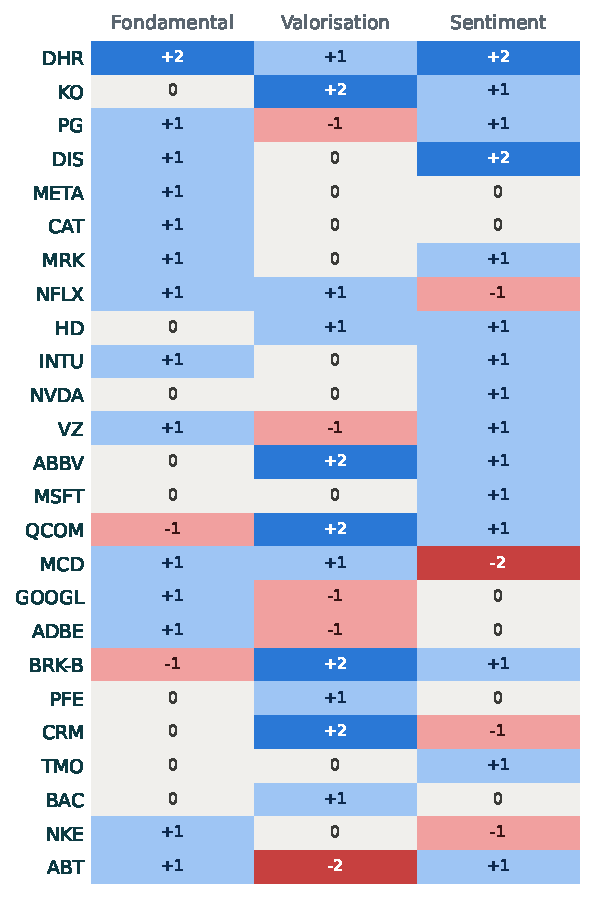
\includegraphics[width=0.55\textwidth]{figures/notes.pdf}
\caption{Notes des trois analystes sur les titres retenus (de $-2$ à $+2$)}
\end{figure}

\section{Allocation}
\begin{figure}[H]
\centering
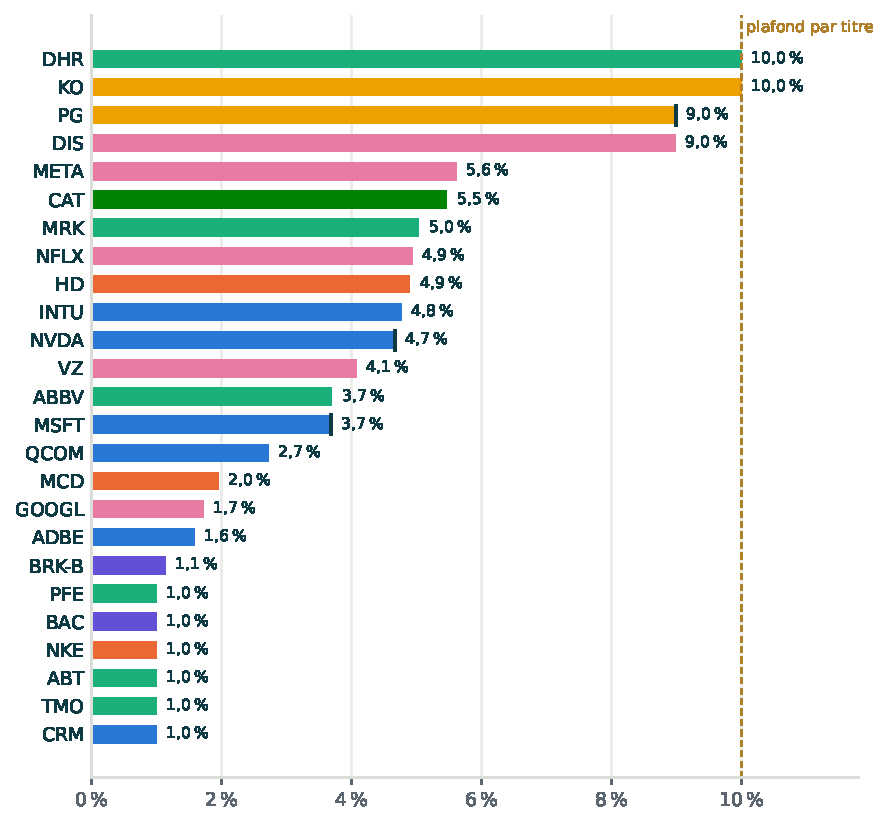
\includegraphics[width=0.88\textwidth]{figures/poids.pdf}
\caption{Poids cible par titre, coloré par secteur ; plafond de 10\,\% par titre}
\end{figure}

\begin{figure}[H]
\centering
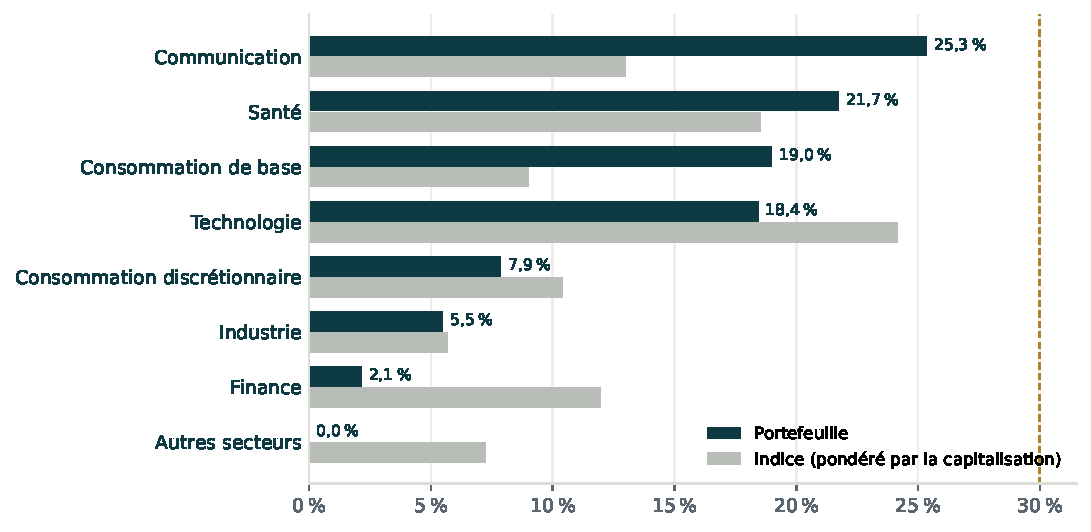
\includegraphics[width=0.88\textwidth]{figures/secteurs.pdf}
\caption{Exposition sectorielle face à l'indice pondéré par la capitalisation}
\end{figure}

\begin{table}[H]
\centering\small
\caption{Principales lignes du portefeuille}
\begin{tabular}{@{}l l r r l@{}}
\toprule
Titre & Secteur & Poids & Vue & Confiance \\
\midrule
\tabinput{tab_allocation.tex}
\bottomrule
\end{tabular}
\end{table}

\section{Effet des vues : Black-Litterman}
\begin{figure}[H]
\centering
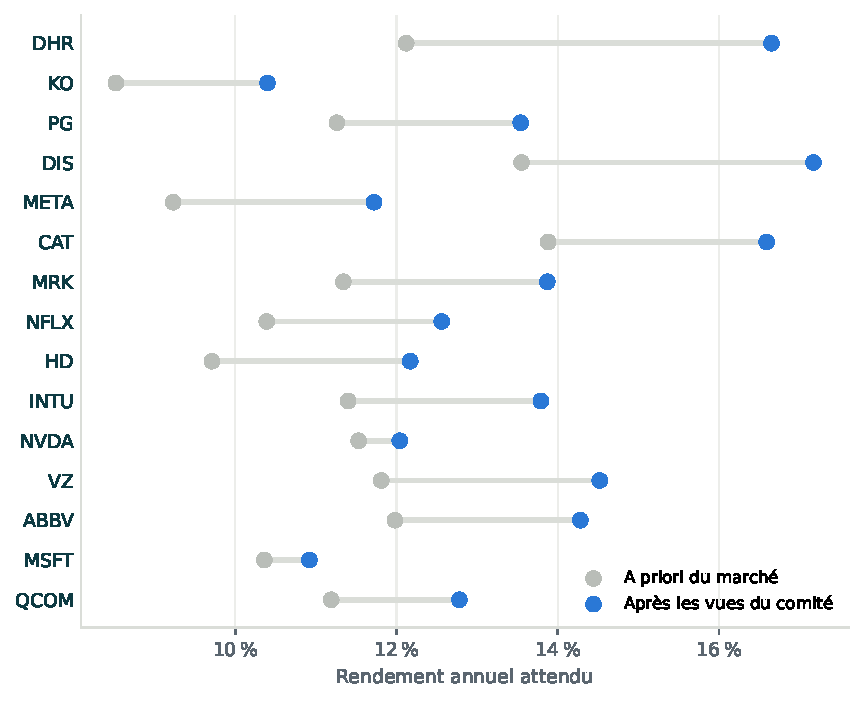
\includegraphics[width=0.85\textwidth]{figures/black_litterman.pdf}
\caption{Rendements attendus avant et après intégration des vues du comité}
\end{figure}

\begin{table}[H]
\centering\small
\caption{Des vues du comité aux rendements a posteriori}
\begin{tabular}{@{}l r l r r r@{}}
\toprule
Titre & Vue & Confiance & A priori & A posteriori & Poids \\
\midrule
\tabinput{tab_bl.tex}
\bottomrule
\end{tabular}
\end{table}

\section{Risque}
\begin{figure}[H]
\centering
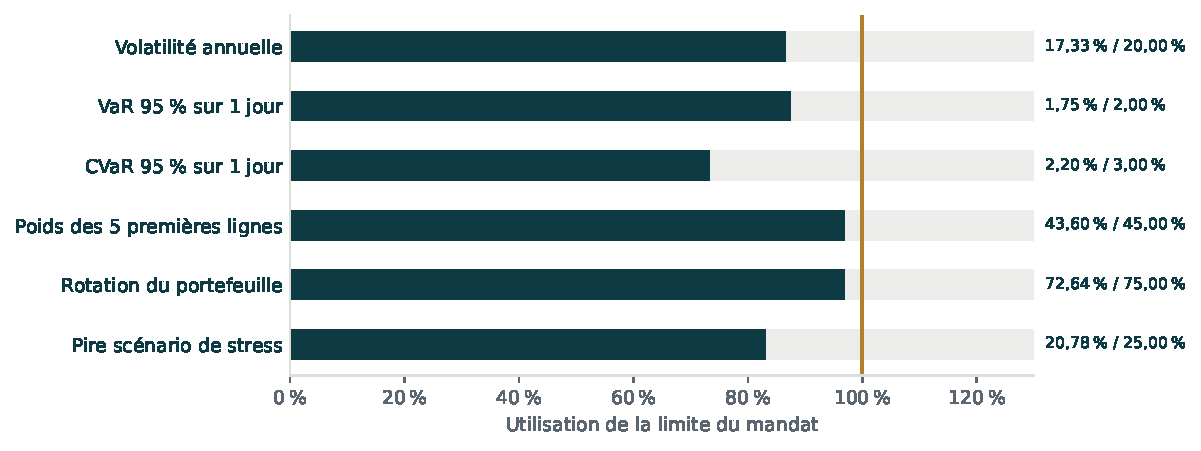
\includegraphics[width=0.85\textwidth]{figures/risque.pdf}
\caption{Utilisation des limites de risque du mandat (trait doré : 100\,\% de la limite)}
\end{figure}

\begin{table}[H]
\centering\small
\caption{Mesures de risque et limites du mandat}
\begin{tabular}{@{}l r r l@{}}
\toprule
Indicateur & Mesure & Limite & Statut \\
\midrule
\tabinput{tab_risque.tex}
\bottomrule
\end{tabular}
\qquad
\begin{tabular}{@{}l r@{}}
\toprule
Scénario de stress & Perte \\
\midrule
\tabinput{tab_stress.tex}
\bottomrule
\end{tabular}
\end{table}

\begin{figure}[H]
\centering
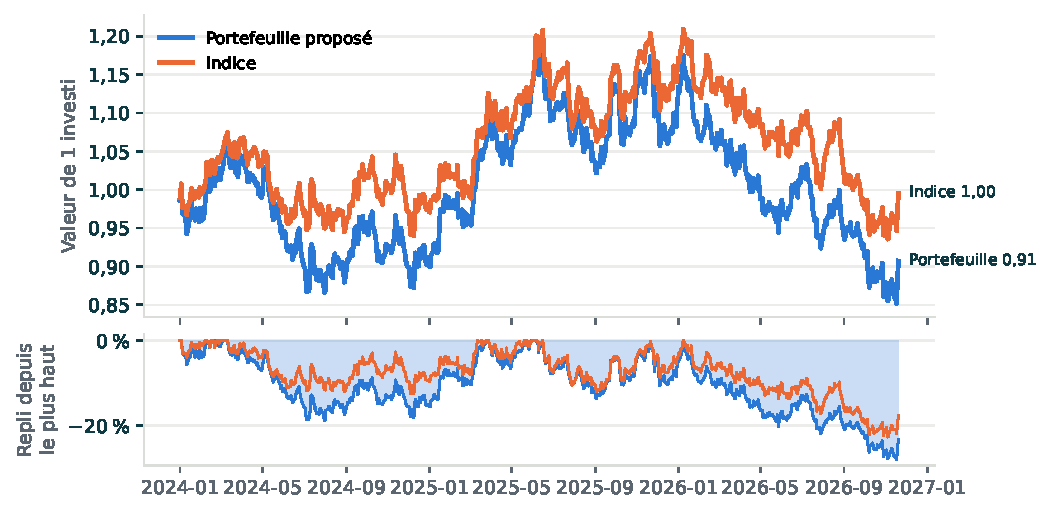
\includegraphics[width=0.9\textwidth]{figures/performance.pdf}
\caption{Comportement passé de l'allocation proposée et repli depuis le plus haut (dans l'échantillon)}
\end{figure}
Sur la période, l'allocation proposée réalise \PerfPortefeuille{} contre \PerfIndice{} pour l'indice. Ce calcul est
effectué \emph{dans l'échantillon} : les poids sont choisis avec ces mêmes données, il ne s'agit donc pas d'une mesure
de performance. Une évaluation rigoureuse exige un backtest point-in-time (chapitre~\ref{ch:limites}).

% =====================================================================
\chapter{Limites et perspectives}\label{ch:limites}

\section{Limites}
\begin{itemize}
  \item \textbf{Données} : yfinance est réservé au prototypage et ses ratios ne sont pas point-in-time ; un fournisseur
        sous licence est nécessaire pour un usage professionnel et pour le marché marocain.
  \item \textbf{Évaluation} : aucune mesure de performance hors échantillon n'est encore produite.
  \item \textbf{Modèles} : les petits modèles ouverts peuvent produire des sorties invalides ; les garde-fous en code
        et le repli par règles limitent l'impact, mais la qualité des thèses dépend du modèle.
  \item \textbf{Coût} : trois agents par titre, soit environ une minute par titre sur un GPU T4 ; l'univers complet
        de 300 titres demande un budget de calcul supérieur.
  \item \textbf{Paramètres} : $\kappa$, $\delta$, les poids des notes et les seuils de risque sont des hypothèses à
        calibrer avec les gérants.
\end{itemize}

\section{Perspectives}
\begin{itemize}
  \item Backtest mensuel point-in-time sur plusieurs années, avec coûts de transaction, et comparaison à des
        portefeuilles de référence (équipondéré, minimum variance, indice).
  \item Évaluation des agents : cohérence des notes dans le temps, pouvoir prédictif des vues, ablation du débat.
  \item Calibration de $\kappa$ et de la confiance à partir de l'historique des vues.
  \item Adaptation au marché marocain (Bourse de Casablanca, AMMC) et extraction des états financiers PDF.
  \item Mémoire des cycles précédents pour que le comité tienne compte de ses décisions passées.
\end{itemize}

% =====================================================================
\chapter*{Conclusion}
\addcontentsline{toc}{chapter}{Conclusion}
Ce projet montre qu'il est possible de tirer parti des modèles de langage pour la sélection de titres sans leur confier
les calculs ni la décision. L'architecture multi-agent, orchestrée par LangGraph, reproduit le fonctionnement d'un
comité d'investissement : analyses spécialisées en parallèle, débat contradictoire, arbitrage, puis passage par des
méthodes quantitatives robustes (rétrécissement de Ledoit-Wolf, Black-Litterman, optimisation sous contraintes) et par
un contrôle des risques systématique. La validation humaine, l'observabilité et le journal d'audit rendent chaque
décision explicable. Le prototype, entièrement open source, constitue une base solide pour une évaluation hors
échantillon et une adaptation au marché marocain.

% =====================================================================
\begin{thebibliography}{99}
\addcontentsline{toc}{chapter}{Bibliographie}
\bibitem{markowitz} H.~Markowitz. Portfolio Selection. \emph{The Journal of Finance}, 7(1):77--91, 1952.
\bibitem{sharpe} W.~F.~Sharpe. Mutual Fund Performance. \emph{The Journal of Business}, 39(1):119--138, 1966.
\bibitem{ledoitwolf} O.~Ledoit et M.~Wolf. Honey, I Shrunk the Sample Covariance Matrix. \emph{The Journal of Portfolio Management}, 30(4):110--119, 2004.
\bibitem{blacklitterman} F.~Black et R.~Litterman. Global Portfolio Optimization. \emph{Financial Analysts Journal}, 48(5):28--43, 1992.
\bibitem{idzorek} T.~Idzorek. A Step-by-Step Guide to the Black-Litterman Model. Zephyr Associates, 2005.
\bibitem{cvar} R.~T.~Rockafellar et S.~Uryasev. Optimization of Conditional Value-at-Risk. \emph{Journal of Risk}, 2(3):21--41, 2000.
\bibitem{finbert} D.~Araci. FinBERT: Financial Sentiment Analysis with Pre-trained Language Models. arXiv:1908.10063, 2019.
\bibitem{bloomberggpt} S.~Wu et al. BloombergGPT: A Large Language Model for Finance. arXiv:2303.17564, 2023.
\bibitem{react} S.~Yao et al. ReAct: Synergizing Reasoning and Acting in Language Models. \emph{ICLR}, 2023.
\bibitem{rag} P.~Lewis et al. Retrieval-Augmented Generation for Knowledge-Intensive NLP Tasks. \emph{NeurIPS}, 2020.
\bibitem{tradingagents} Y.~Xiao, E.~Sun, D.~Luo et W.~Wang. TradingAgents: Multi-Agents LLM Financial Trading Framework. arXiv:2412.20138, 2024.
\bibitem{qwen} Qwen Team. Qwen2.5 Technical Report. arXiv:2412.15115, 2024.
\bibitem{langgraph} LangChain. LangGraph documentation. \url{https://langchain-ai.github.io/langgraph/}.
\end{thebibliography}

% =====================================================================
\appendix
\chapter{Mandat de démonstration}
\begin{lstlisting}
contraintes:
  long_only: true
  poids_max_titre: 0.10
  poids_min_ligne: 0.01
  poids_max_secteur: 0.30
  liquidite_min_usd_jour: 50000000
  capitalisation_min_usd: 20000000000
limites_risque:
  volatilite_annuelle_max: 0.20
  var95_1j_max: 0.020
  cvar95_1j_max: 0.030
  rotation_max: 0.75
  concentration_top5_max: 0.45
  perte_stress_max: 0.25
\end{lstlisting}

\chapter{Reproduire les résultats}
\begin{lstlisting}
pip install -r requirements.txt
pytest -q                                   # tests hors ligne
python docs/rapport/generer_figures.py --backend ollama --source yfinance
pdflatex rapport.tex && pdflatex rapport.tex
streamlit run app/streamlit_app.py          # interface du comité
\end{lstlisting}

\end{document}
